\chapter{Python}
\thispagestyle{fancy}
\lstset{language=Python}

The official python documentation can be found at the following links
\begin{lstlisting}
# Documentation for version 3+
https://docs.python.org/3/
# Documentation for version 2+
https://docs.python.org/2/
\end{lstlisting}

Import floating point division which allows python 2 compatibility when using division with doubles. Include this at the beginning of the script.
\begin{lstlisting}
from __future__ import division
\end{lstlisting}

\section{Plotting and Graphs\index{Plotting and Graphs}}

A nicely formatted plot with a legend using the pylab package.
\begin{lstlisting}
import pylab as plt #Imports the correct packages for plotting.

plt.title('Contamination & Beam Health % vs Time') # Creates a title.

plt.plot(t, Contamination, '-b', label='Contamination') #Plots Contamination in blue.
plt.plot(t, Beam_loss, '-r', label='Beam Loss') #Plots Beam_loss in red.
plt.plot(t, Beam_health, '-g', label='Beam Health') #Plots Beam_health in green.
#plt.plot(x,y,'-color', label='Legend Label') #Template

plt.xlabel("time (seconds)") #Creates a x-axis label
plt.ylabel("Contamination %") #Creates a y-axis label

plt.legend(loc='center right') #Creates a legend with the labels set above.
#Other locations include upper/lower/center left/right

plt.show() #Displays plot.
\end{lstlisting}
This code would display a graph such as the one below such that the proper values are input.

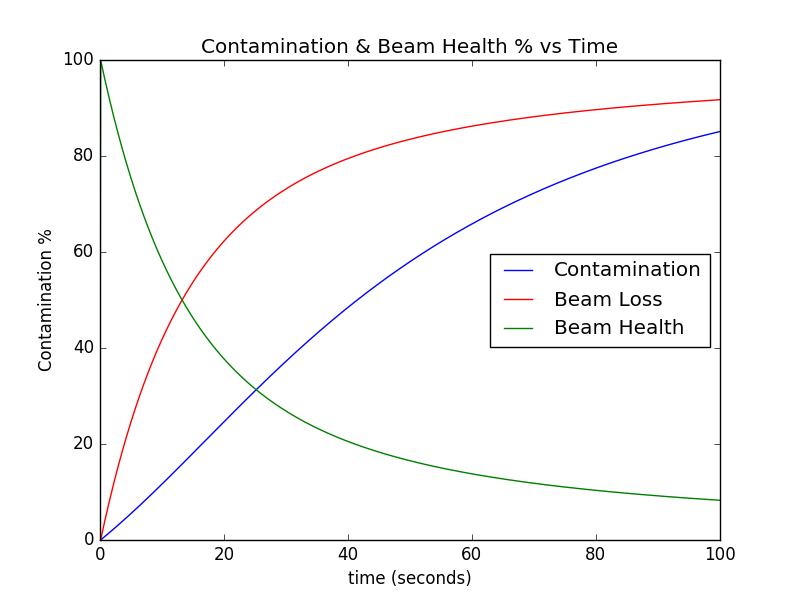
\includegraphics[width=0.5\linewidth]{./Images/Figures/figure_1-4}


